\section{Wolfenstein 3D-VR}
Around 1994 a company called Alternate World Technologies worked on an adaptation of the Wolfenstein 3D engine, designed to work with head-mounted displays, under special license from id Software. AWT worked on three games: Wolfenstein VR, Blake Stone VR, and Cybertag VR, all based on the Wolfenstein engine code, with Cybertag being the only one playable in multiplayer for up to four players. A 3D artist by the name of Tom Roe, who uploaded a video on youtube\footnote{https://www.youtube.com/watch?v=l9n\_TkFIttk}, helped with some of the finer details of this project.\\

\begin{fancyquotes}
The Wolfenstein VR game was developed by a small game development company based in Louisville, KY back in 1993. Through an agreement with Id, Alternate Worlds Technologies, Inc., (AWT) licensed the original Wolfenstein 3D engine and used Polhemus tracker technology to create a head mounted display version of the game. The design team also modified all of the animation sequences to look more like green alien blood rather than red blood; an attempt to reduce the apparent violence in the game. Amusing by today's standards for sure.
 \bigskip \\
I was not personally involved in the design work on Wolfenstein as I arrived after they were already shipping arcade units with this title. They also created a similar experience with Blake Stone. The Wolfenstein VR game was a single player game, though the Wolfenstein engine was later used to create a multi-player game which you mentioned, Cybertag VR. Where four players could speak to each other through a headset while playing tag in a virtual environment. I began my work with AWT as a 3d artist developing levels for a new game engine which used character and level models designed in 3d Studio. I also used Deluxe Paint to create animation sequences for Cybertag VR.
 \bigskip \\
\textbf{Tom Roe - 3D artist}
 \end{fancyquotes}


Trivia: Wolfenstein VR remains on the MAME project's "Undumped" list to this day.

\begin{figure}[H]
  \centering
 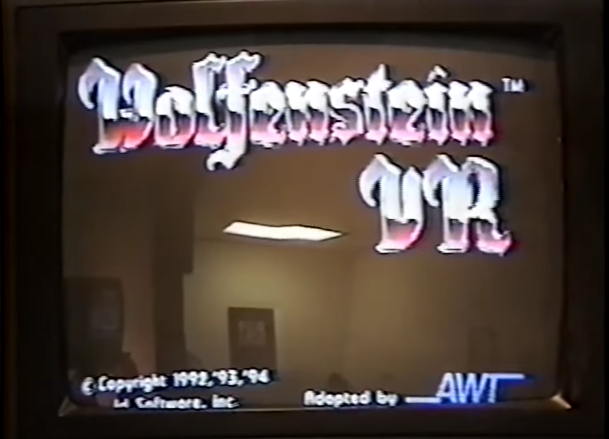
\includegraphics[width=\textwidth]{screenshots/w3dvr/title.png}
 \caption{Title screen}
\end{figure}

\begin{figure}[H]
  \centering
 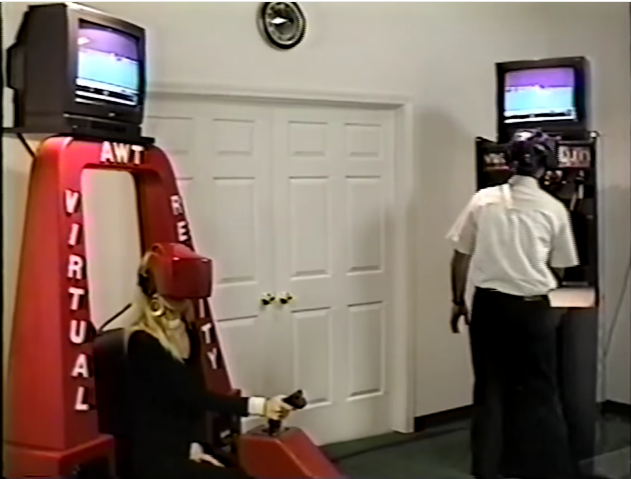
\includegraphics[width=\textwidth]{screenshots/w3dvr/multiplayer.png}
 \caption{Title screen}
\end{figure}

\begin{figure}[H]
  \centering
 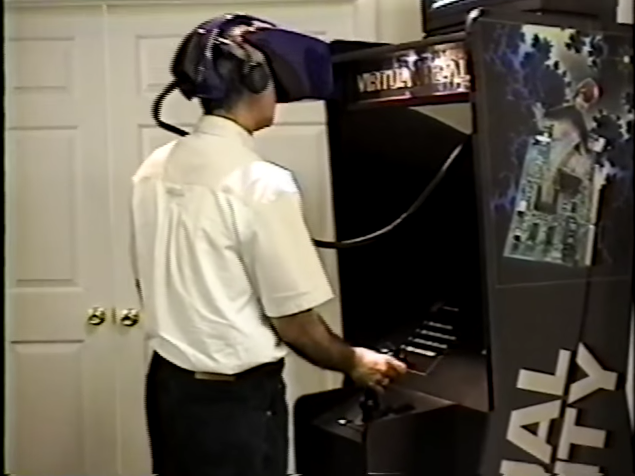
\includegraphics[width=\textwidth]{screenshots/w3dvr/station.png}
 \caption{Title screen}
\end{figure}

\begin{figure}[H]
  \centering
 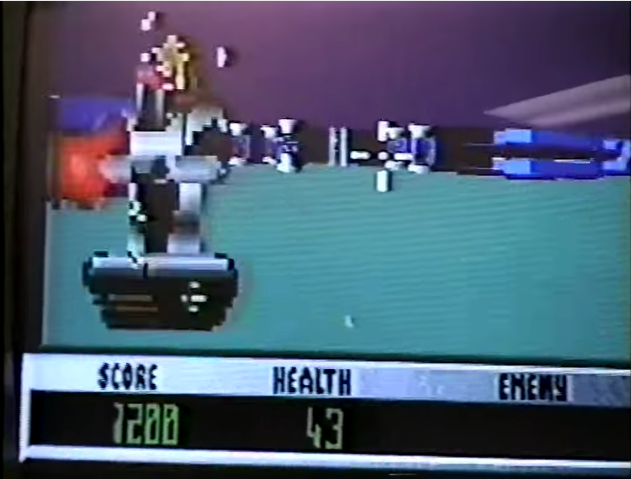
\includegraphics[width=\textwidth]{screenshots/w3dvr/game.png}
 \caption{Title screen}
\end{figure}


